%! TEX rootmain.tex

\chapter{Reed and Lip Excitation}

In many wind instruments, sound is produced by the interaction between a quasi-steady air supply and a vibrating element that behaves as a valve. Reeds and lips can be treated as pressure-controlled valves, whose motion is driven by the pressure difference across the valve and whose vibration is shaped by the coupling with the instrument air column. The chapter first introduces a practical classification of these valves and a qualitative overview of the sound-generation mechanism. It then moves to reed modeling, discusses the role of nonlinearities in enabling self-oscillations, and interprets the reed as an acoustic generator coupled to a resonator. Finally, the large-amplitude regime is addressed, where the valve motion and the resulting flow modulation depart significantly from small-signal behavior.

\section{Valve Categories}

\subsection{Pressure-controlled Valves}

Several wind-instrument exciters can be regarded as pressure-controlled valves. Examples include single-reed systems such as the clarinet or saxophone, double reeds such as the oboe or bassoon, organ-reed pipes, and the player’s lips in brass instruments. In all cases, the valve motion is controlled by the pressure difference across the valve. The vibration frequency is controlled partly by the natural frequency of the reed and partly by the resonances of the instrument air column to which it is connected. A compact overview of common pressure-controlled valves is shown in figure \ref{fig:valve_categories_overview}.

\begin{figure}[!htb]
\centering
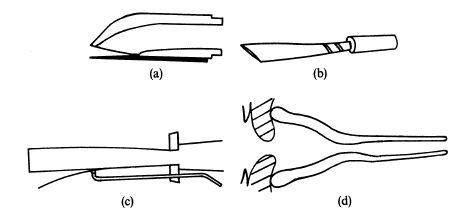
\includegraphics[width=0.7\linewidth]{00_Images/04_chapter/img28.jpg}
\caption{Examples of pressure-controlled valves used in wind instruments}
\label{fig:valve_categories_overview}
\end{figure}

\paragraph{Valve classification} A compact classification is obtained by introducing the doublet symbol \( (\sigma_1,\sigma_2) \), defined by the effect of steady pressure applied at the inlet and at the outlet:
\[
\begin{aligned}
\sigma_1 &= +1 && \text{if a pressure excess at the inlet tends to open the valve} \\
\sigma_1 &= -1 && \text{otherwise} \\
\sigma_2 &= +1 && \text{if a pressure excess at the outlet tends to open the valve} \\
\sigma_2 &= -1 && \text{otherwise}
\end{aligned}
\]
The classification can be visualized schematically as in figure \ref{fig:valve_classification_sigma}.

\begin{figure}[!htb]
\centering
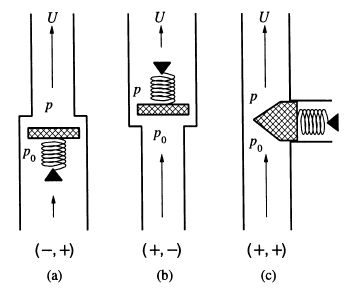
\includegraphics[width=0.7\linewidth]{00_Images/04_chapter/img63.jpg}
\caption{Valve classification based on the doublet \((\sigma_1,\sigma_2)\)}
\label{fig:valve_classification_sigma}
\end{figure}

\paragraph{Three valve types} Within this framework, three relevant valve types are distinguished:

\begin{itemize}
    \item \( (-,+) \): inward-striking valve, associated with woodwind reeds
    \item \( (+,-) \): outward-striking valve, associated with the player’s lips in one brass instrument model
    \item \( (+,+) \): sideways-striking valve, associated with the player’s lips in an alternative brass instrument model
\end{itemize}

The combination \( (-,-) \) is not useful in this context. The three relevant valve types are illustrated in figure \ref{fig:three_valve_types}.

\begin{figure}[!htb]
\centering
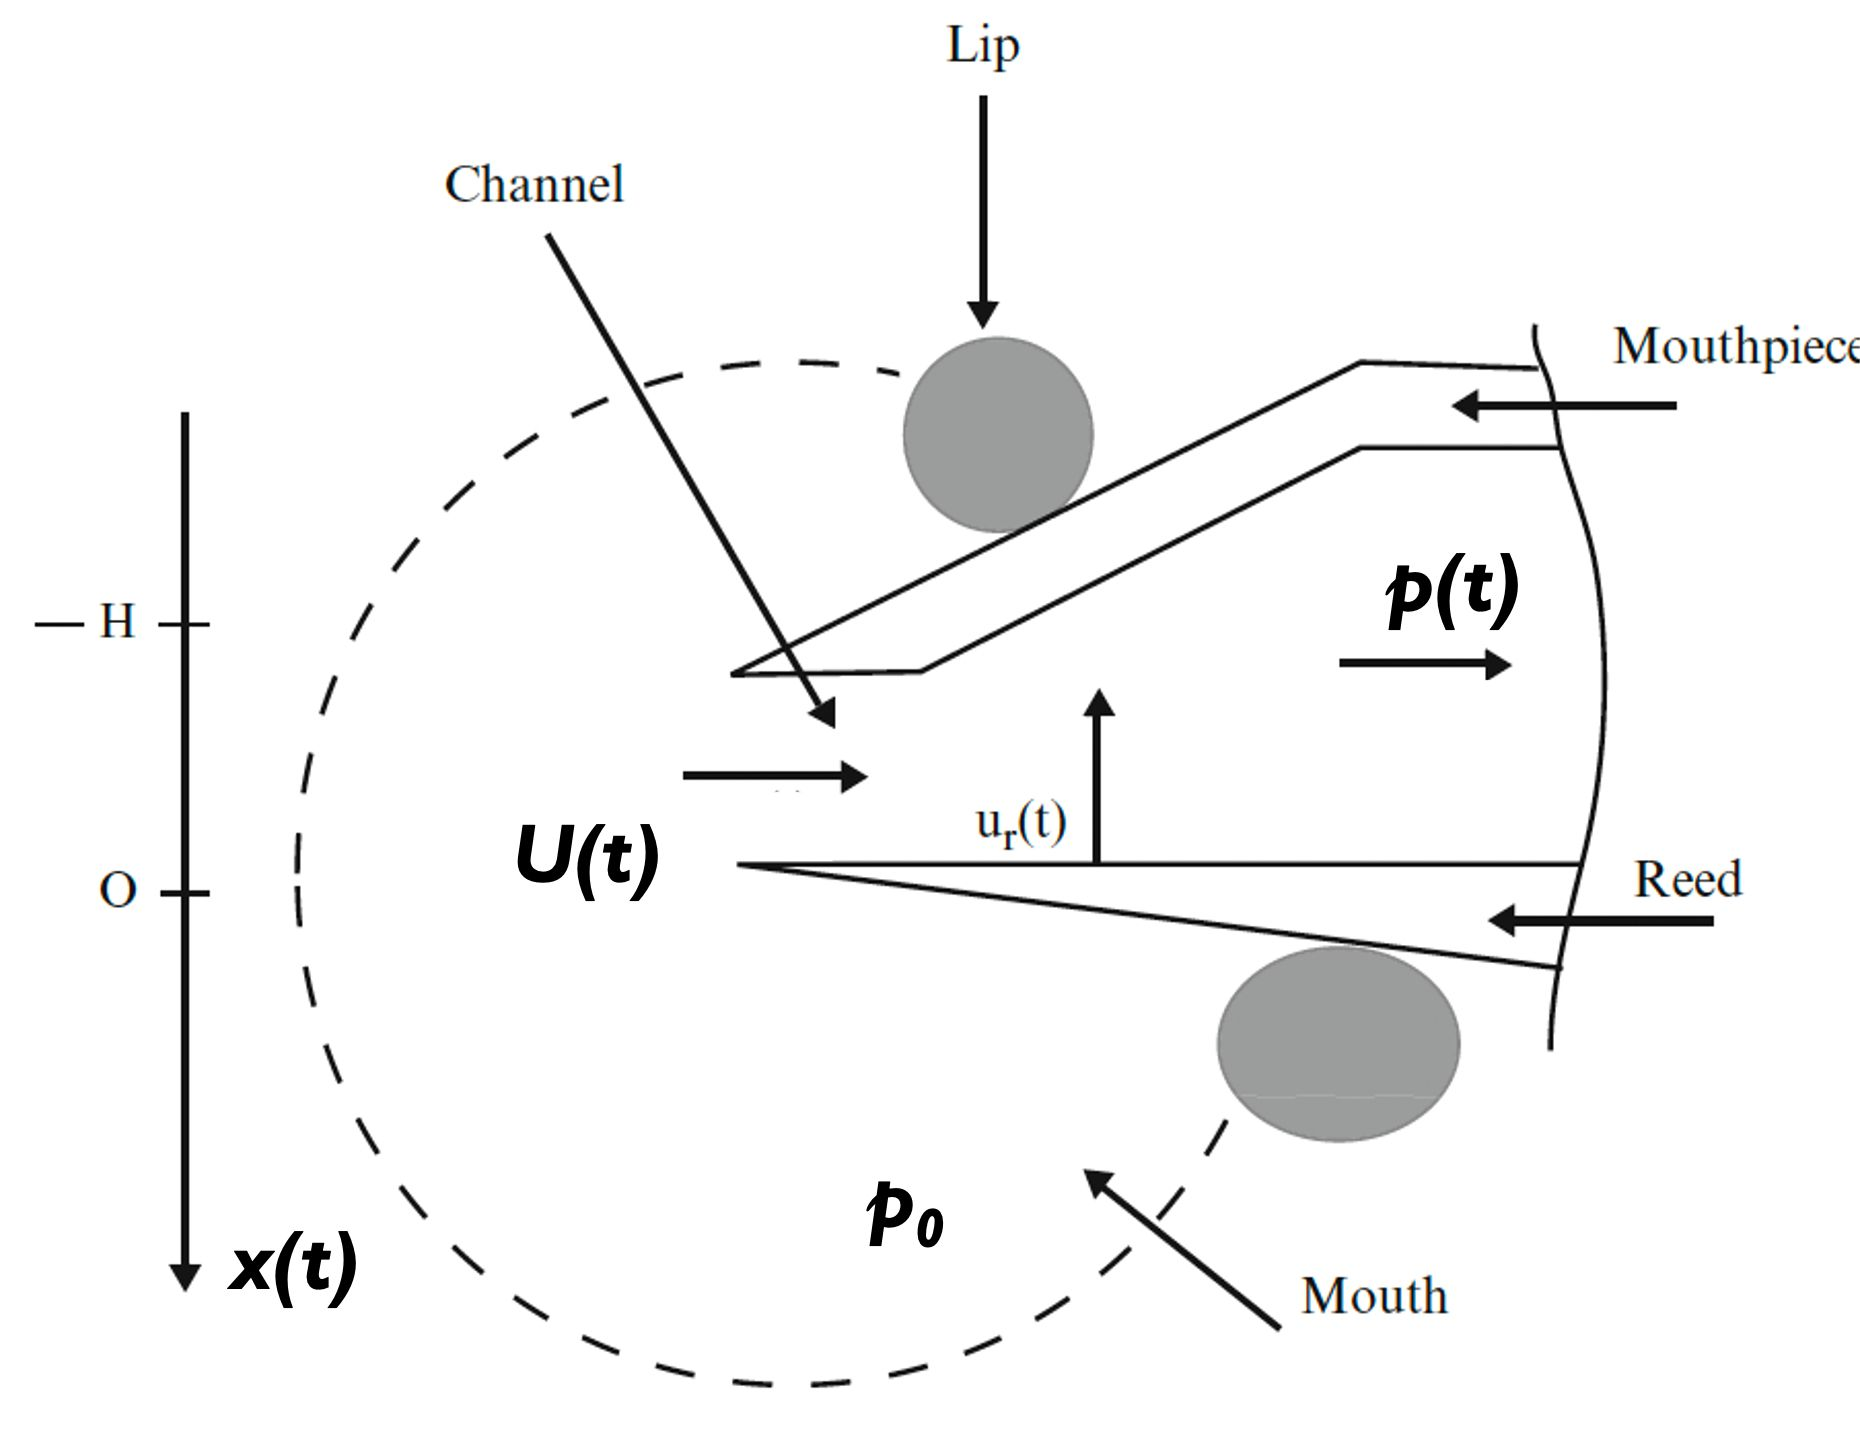
\includegraphics[width=0.7\linewidth]{00_Images/04_chapter/img73.jpg}
\caption{Inward-, outward-, and sideways-striking valve configurations}
\label{fig:three_valve_types}
\end{figure}

\subsection{Sound Generation in a Nutshell}

Blowing into the mouthpiece displaces the reed from its rest position. Because the reed is elastic, it tends to restore the displacement and can exhibit a complex oscillatory motion. This oscillation perturbs the air column in the reed channel and in the resonator. The resonance frequency is determined jointly by the elastic properties of the reed and the air column, indicating strong coupling between the mouthpiece and the resonator.

\subsection{Clarinet Reed}

The clarinet reed configuration is illustrated through lateral and top or bottom views, highlighting the reed geometry and its placement relative to the mouthpiece. Representative views of the clarinet reed geometry are given in figure \ref{fig:clarinet_reed_views}.

\begin{figure}[!htb]
\centering
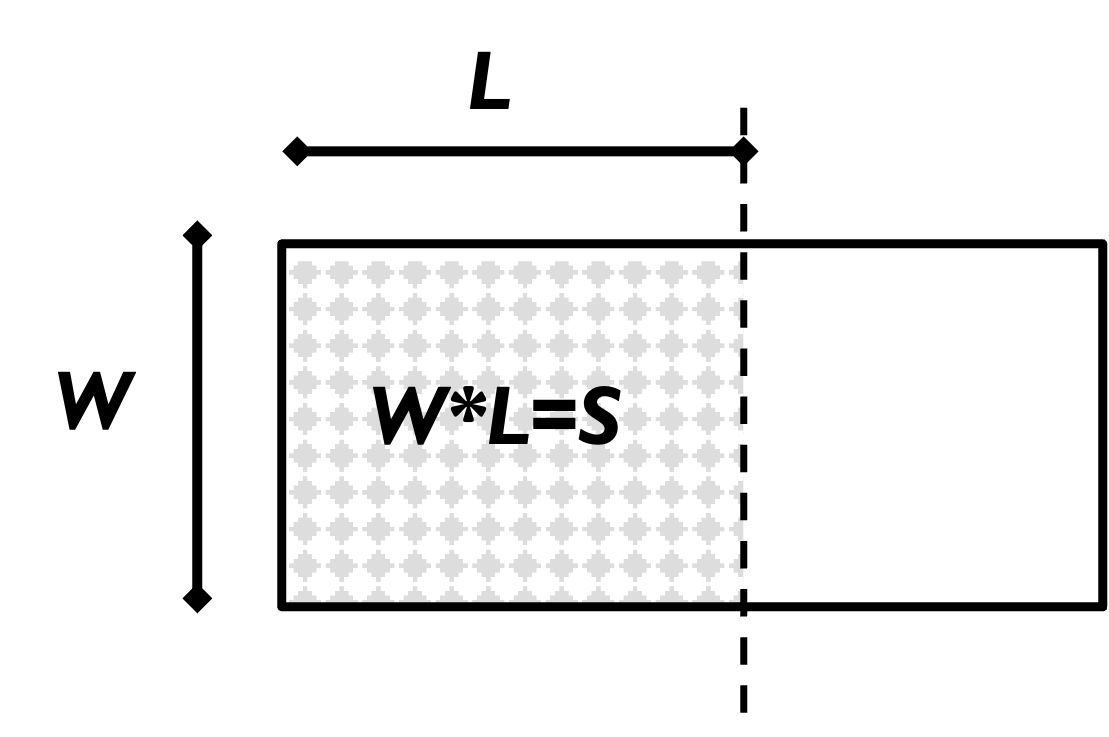
\includegraphics[width=0.6\linewidth]{00_Images/04_chapter/img75.jpg}
\caption{Clarinet reed geometry and placement relative to the mouthpiece}
\label{fig:clarinet_reed_views}
\end{figure}

\subsection{Lip Valves}

For lip valves, an excess of pressure at the inlet determines an opening of the valve, corresponding to \( \sigma_1 = +1 \). An excess of pressure at the outlet also determines an opening of the valve, corresponding to \( \sigma_2 = +1 \). A schematic representation of lip-valve operation is shown in figure \ref{fig:lip_valves_scheme}.

\begin{figure}[!htb]
\centering
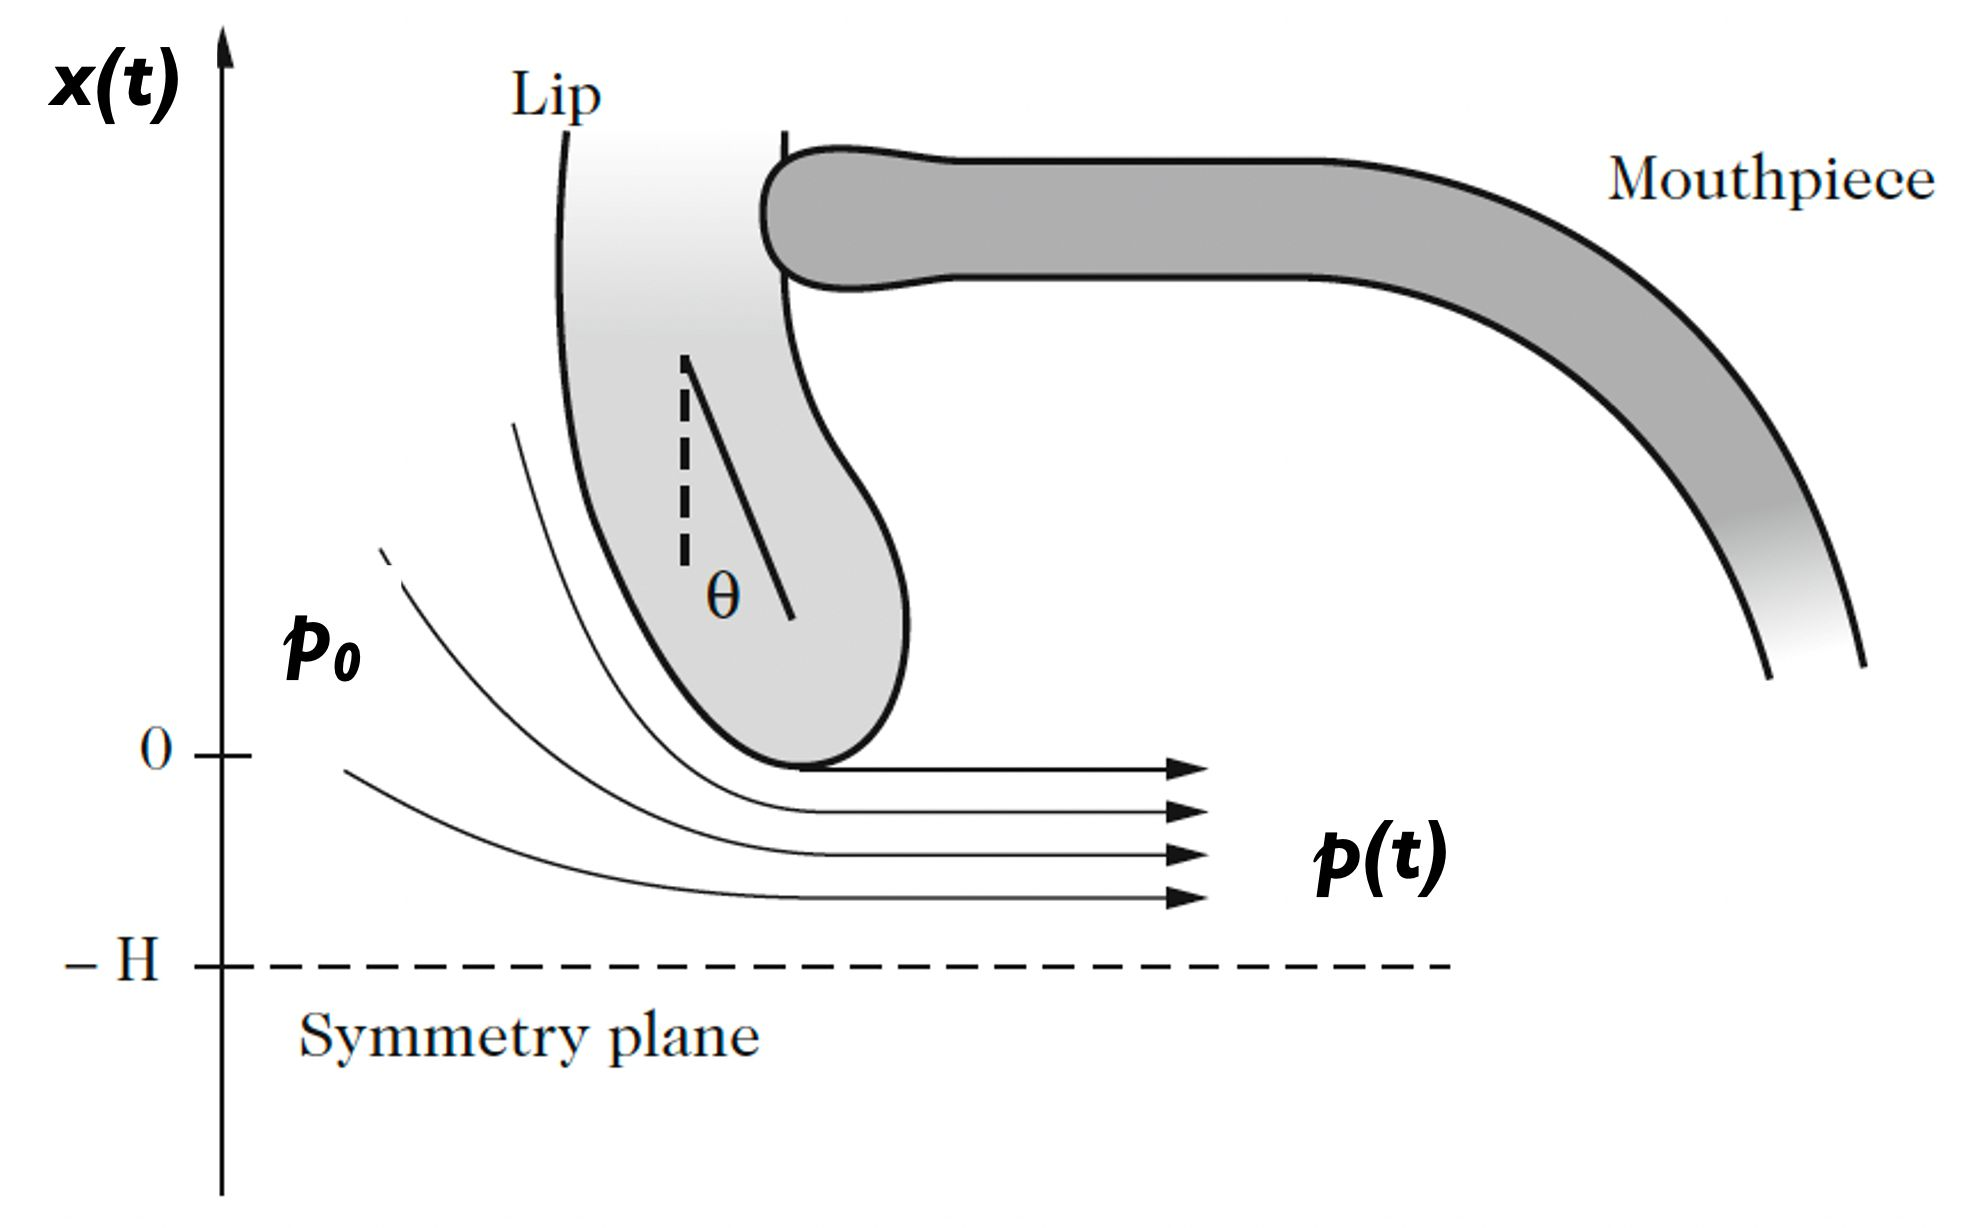
\includegraphics[width=0.6\linewidth]{00_Images/04_chapter/img82.jpg}
\caption{Lip valve as a pressure-controlled valve}
\label{fig:lip_valves_scheme}
\end{figure}

\section{Reed Quasi-static Modeling}

A first description of reed excitation can be built from a quasi-static flow model. Under the assumption of incompressible flow, Bernoulli’s principle relates flow speed and pressure along a streamline through
\[
\frac{v^2}{2} + gz + \frac{p}{\rho} = \text{const}
\]
where \( v \) is the flow speed, \( p \) the static pressure, \( \rho \) the fluid density, \( g \) the gravitational acceleration, and \( z \) the elevation. 

\paragraph{Flow through a valve} Consider a steady flow through a valve driven by an upstream pressure \( p_0 \) and an outlet pressure \( p \). Let \( x \) be the valve opening and \( W \) its width. After standard simplifications, the pressure drop \( p_0 - p \) can be related to the flow speed as
\[
p_0 - p = \frac{\rho v^2}{2}
\qquad
\Rightarrow
\qquad
v = \sqrt{\frac{2(p_0 - p)}{\rho}}
\]
so that the acoustic volume flow becomes
\[
U = Wxv = Wx\sqrt{\frac{2(p_0 - p)}{\rho}}
\]

\paragraph{Static reed opening} To close the model, the reed is represented as a spring with compliance \( C \). Denoting by \( x_0 \) the opening at rest and by \( S \) the effective reed area, the static deflection is written as
\[
x_0 - x = (\sigma_1 p_0 + \sigma_2 p)SC
\]
so that, after substitution into the expression for \( U \),
\[
U = W\left[x_0 - (\sigma_1 p_0 + \sigma_2 p)SC\right]\sqrt{\frac{2(p_0 - p)}{\rho}}
\]
This construction includes only a static force balance, and therefore defines a static reed model. 

\paragraph{Woodwind reed characteristic} For a woodwind reed, \( \sigma_1 = -1 \) and \( \sigma_2 = 1 \), which yields a characteristic of the form
\[
U = \sqrt{\alpha(p_0 - p)} - \sqrt{\beta(p_0 - p)^3}
\]
with constants \( \alpha \) and \( \beta \) collecting the geometric and mechanical parameters of the valve. The resulting \( (p_0 - p, U) \) characteristic is typically represented as a curve with distinct operating regions. A typical static characteristic for a woodwind reed, with the usual operating points, is shown in figure \ref{fig:woodwind_characteristic_OABC}.

\begin{figure}[!htb]
\centering
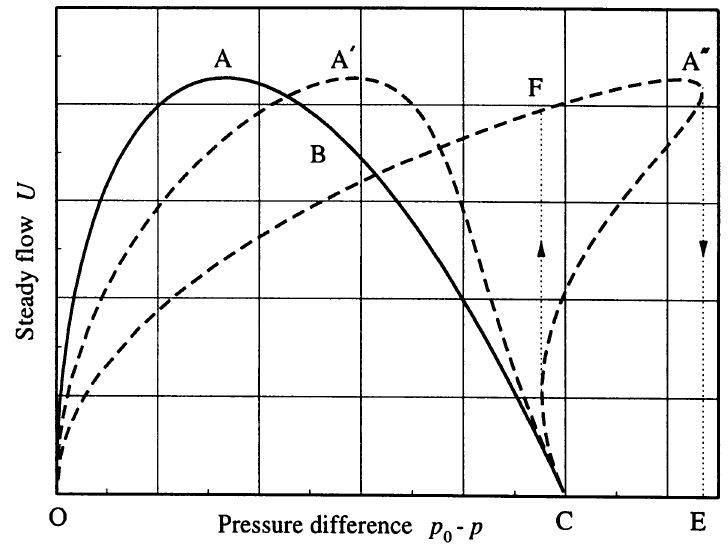
\includegraphics[width=0.7\linewidth]{00_Images/04_chapter/img99.jpg}
\caption{Woodwind reed quasi-static characteristic with operating regions}
\label{fig:woodwind_characteristic_OABC}
\end{figure}

\paragraph{Low-frequency admittance and negative resistance} The acoustic admittance presented by the reed to the instrument, at very low frequency, can be inferred from the characteristic curve through the slope
\[
G = \frac{\partial U}{\partial p}
\]
Where this slope is negative, the reed behaves as a negative resistance, namely as a flow generator. In the characteristic construction discussed in the slides, the negative-resistance region extends from A to C, with \( p_A = p_C/3 \), and a convenient operating point is B, for which \( p_B = 2p_C/3 \). 

\paragraph{Double reeds and additional flow resistance} In double-reed instruments such as oboe or bassoon, the narrow passage between the two reeds introduces an additional flow resistance \( R \). Changing \( R \) modifies the \( (p_0 - p, U) \) characteristic: the negative-resistance region can become narrower and steeper, and in some cases hysteresis may appear. The influence of an additional flow resistance on the static characteristic, including possible hysteresis, is illustrated in figure \ref{fig:double_reeds_resistance_effect}.

\begin{figure}[!htb]
\centering
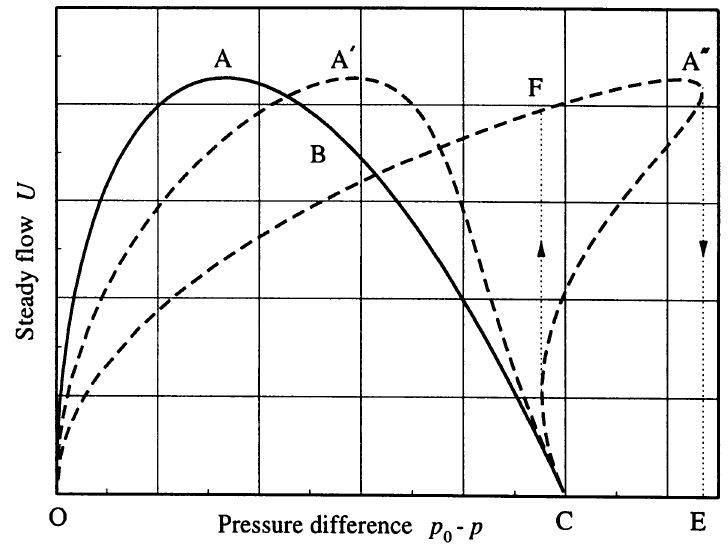
\includegraphics[width=0.7\linewidth]{00_Images/04_chapter/img109.jpg}
\caption{Effect of added flow resistance on the double-reed static characteristic}
\label{fig:double_reeds_resistance_effect}
\end{figure}

\section{Nonlinearities and Self-oscillations}

In instruments with continuous energy input, such as wind and bowed-string instruments, sound generation depends on specific conditions in the exciter-resonator interaction. A central point is that the exciter is typically governed by nonlinear dynamics, so that its input depends on its own state and on the coupled acoustic field. 

\subsection{Nonlinear Dynamic Model}

A generic nonlinear model for the exciter displacement \( y(t) \) can be written as
\[
m\ddot y + R\dot y + Ky = F(y,\dot y,t)
\]
so that the forcing depends on the output \( y \), on its time derivative, and possibly on additional external inputs. Typical examples include bowed strings, where the bow force depends on the relative velocity between bow and string, and reed instruments, where the pressure depends on the reed displacement, which is the unknown function of the differential equation. In addition, \( m \), \( R \), and \( K \) may also depend on \( y \). It is convenient to rewrite the dynamics in the normalized form
\[
\ddot y + \omega_0^2 y = g(y,\dot y,t)
\]
where \( \omega_0 \) is the linear natural frequency and \( g \) collects damping, nonlinearity, and forcing contributions.

\subsection{Slowly Varying Amplitude and Phase}

If damping, nonlinearity, and external forcing are small, the response is approximately sinusoidal,
\[
y(t) = a\sin(\omega_0 t + \phi)
\]
If \( g \neq 0 \) but remains small compared to the linear restoring term, a standard assumption is that amplitude and phase vary slowly in time,
\[
y(t) = a(t)\sin\!\bigl(\omega_0 t + \phi(t)\bigr)
\]
Differentiation yields
\[
\dot y
= \dot a \cos(\omega_0 t + \phi)
+ a(\omega_0 + \dot \phi)\cos\!\bigl(\omega_0 t + \phi(t)\bigr)
\]
A simplification is obtained by imposing the constraint
\[
\dot a \sin(\omega_0 t + \phi) + a\dot \phi \cos(\omega_0 t + \phi) = 0
\]
which leads to
\[
\dot y = a\omega_0 \cos(\omega_0 t + \phi)
\]
Substituting the assumed form for \( y \) and \( \dot y \) into the normalized equation gives
\[
a\omega_0 \dot a \cos(\omega_0 t + \phi) - a\omega_0 \dot \phi \sin(\omega_0 t + \phi) = g
\]
and combining the two relations yields evolution equations for amplitude and phase,
\[
\dot a = \frac{g}{\omega_0}\cos(\omega_0 t + \phi)
\qquad
\dot \phi = -\frac{g}{a\omega_0}\sin(\omega_0 t + \phi)
\]
Neglecting terms whose frequency is comparable with \( \omega_0 \), and retaining only the slowly varying components \( \langle \dot a \rangle \) and \( \langle \dot \phi \rangle \), the instantaneous frequency and amplitude can be expressed as
\[
\omega = \omega_0 + \langle \dot \phi \rangle
\qquad
a(t) = a(t_0) + \int_{t_0}^{t} \langle \dot a \rangle dt
\]
These relations provide a practical characterization once the state at \( t_0 \) is known.

\subsection{Duffing Oscillator}

As an instructive nonlinear example, consider a system with stiffness that changes with displacement, representing a progressively stiffer or weaker spring. In this setting, the normalized model can be interpreted as
\[
\ddot y + \omega_0^2 y = g(y,\dot y,t)
\qquad
g = f(t) - 2\alpha \dot y - \beta y^3
\]
If the external force \( f(t) \) is sinusoidal at frequency \( \omega \), the resulting frequency-amplitude response differs depending on the sign of \( \beta \). A hysteretic behavior may appear in the forced response, with jump phenomena between branches when sweeping frequency. Typical amplitude frequency responses of the Duffing oscillator are shown in figure \ref{fig:duffing_response}.

\begin{figure}[!htb]
\centering
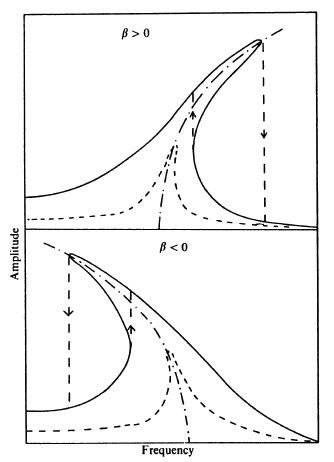
\includegraphics[width=0.6\linewidth]{00_Images/04_chapter/img118.jpg}
\caption{Duffing oscillator: forced response and hysteresis for different nonlinear stiffness signs}
\label{fig:duffing_response}
\end{figure}

\subsection{Self-excitation: Van der Pol Oscillator}

A prototypical self-excited oscillator is obtained with
\[
\ddot y + \omega_0^2 y = g(y,\dot y)
\qquad
g(y,\dot y) = a\dot y(1-y^2)
\]
No external input force is present; yet, oscillations can be sustained. In this model, the effective damping is negative for \( |y|<1 \) and positive for \( |y|>1 \), so that small-amplitude oscillations tend to grow while large-amplitude oscillations are attenuated. For sufficiently small \( a \), the oscillations remain close to sinusoidal. Examples of time histories and phase portraits for the Van der Pol oscillator are shown in figure \ref{fig:vanderpol_examples}.

\begin{figure}[!htb]
\centering
\subfloat{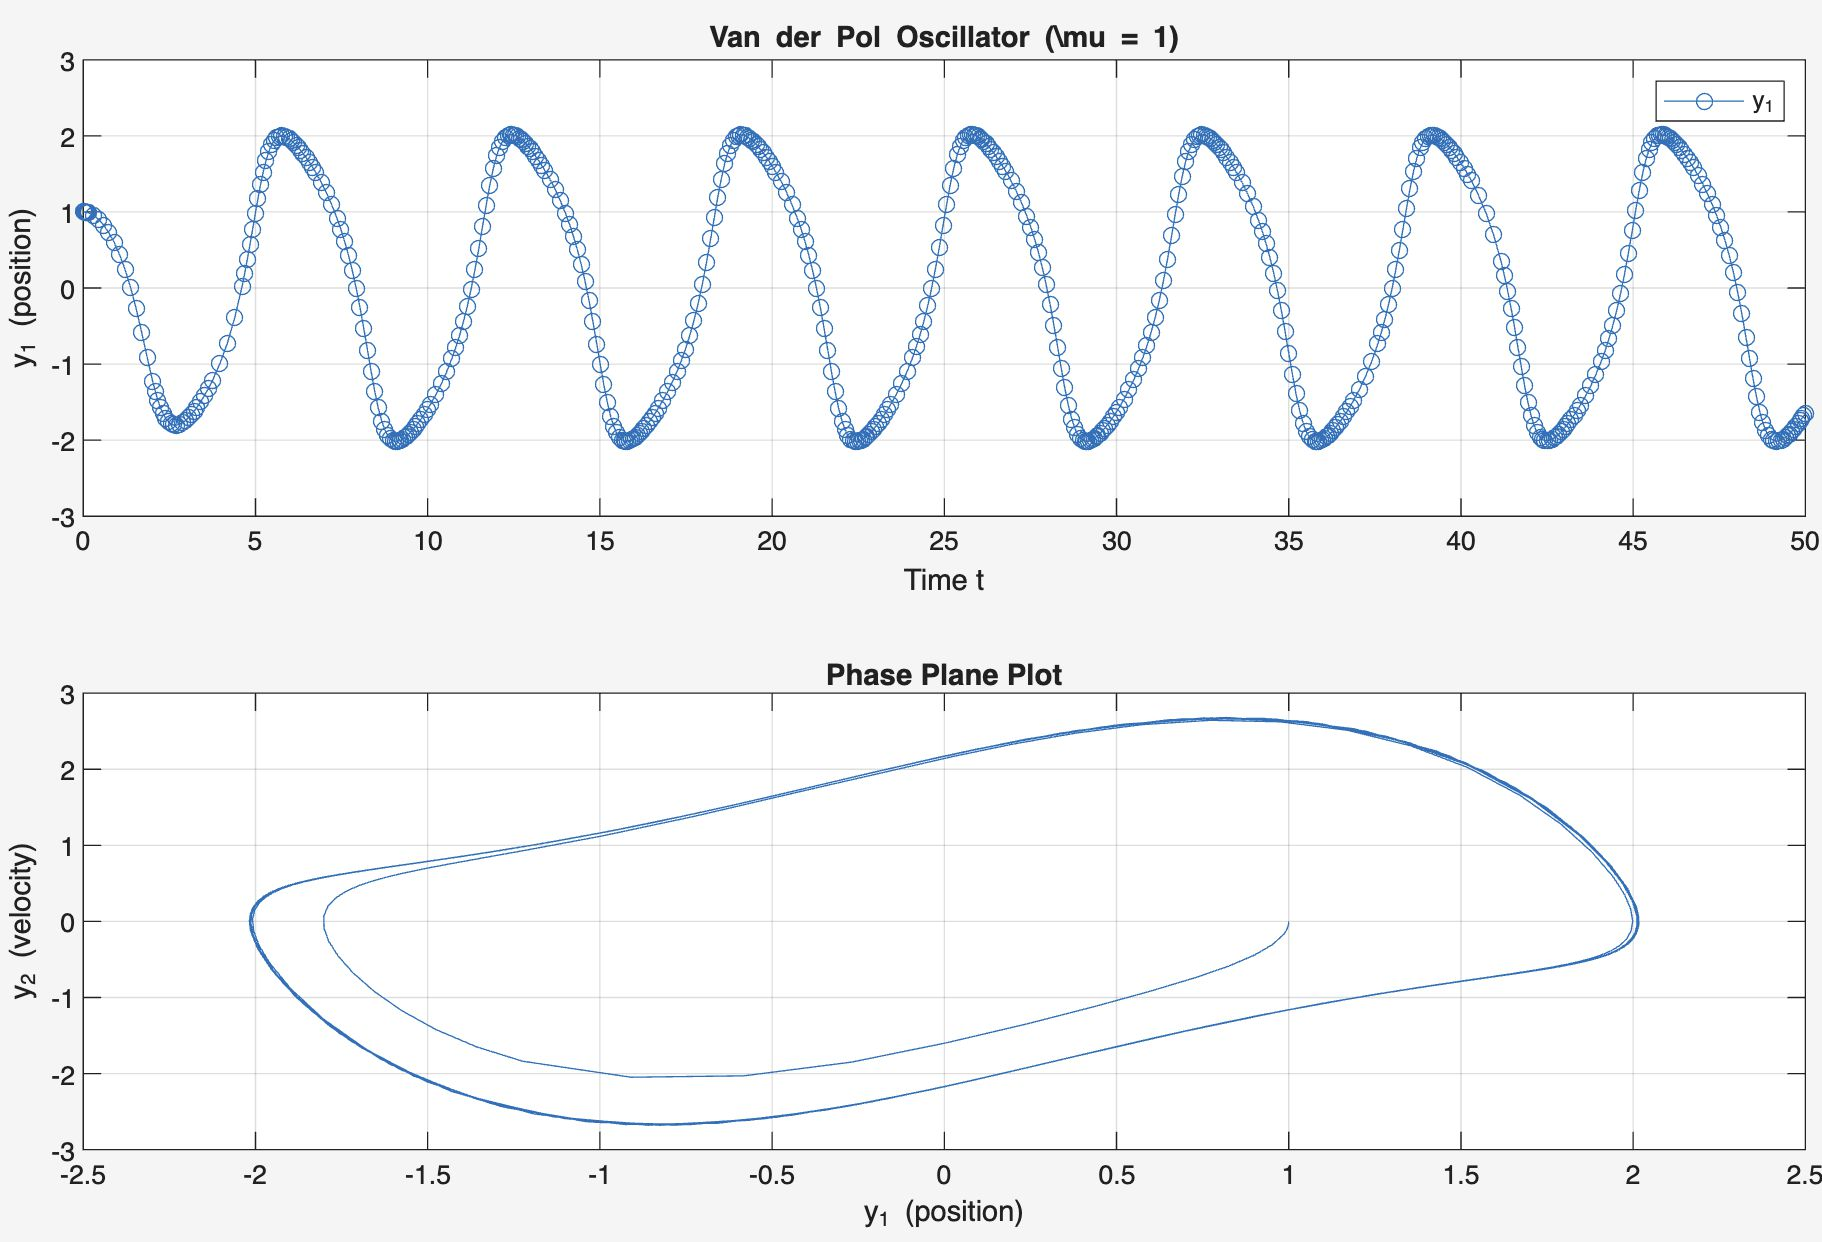
\includegraphics[width=0.45\linewidth]{00_Images/04_chapter/img125.jpg}}\hfill
\subfloat{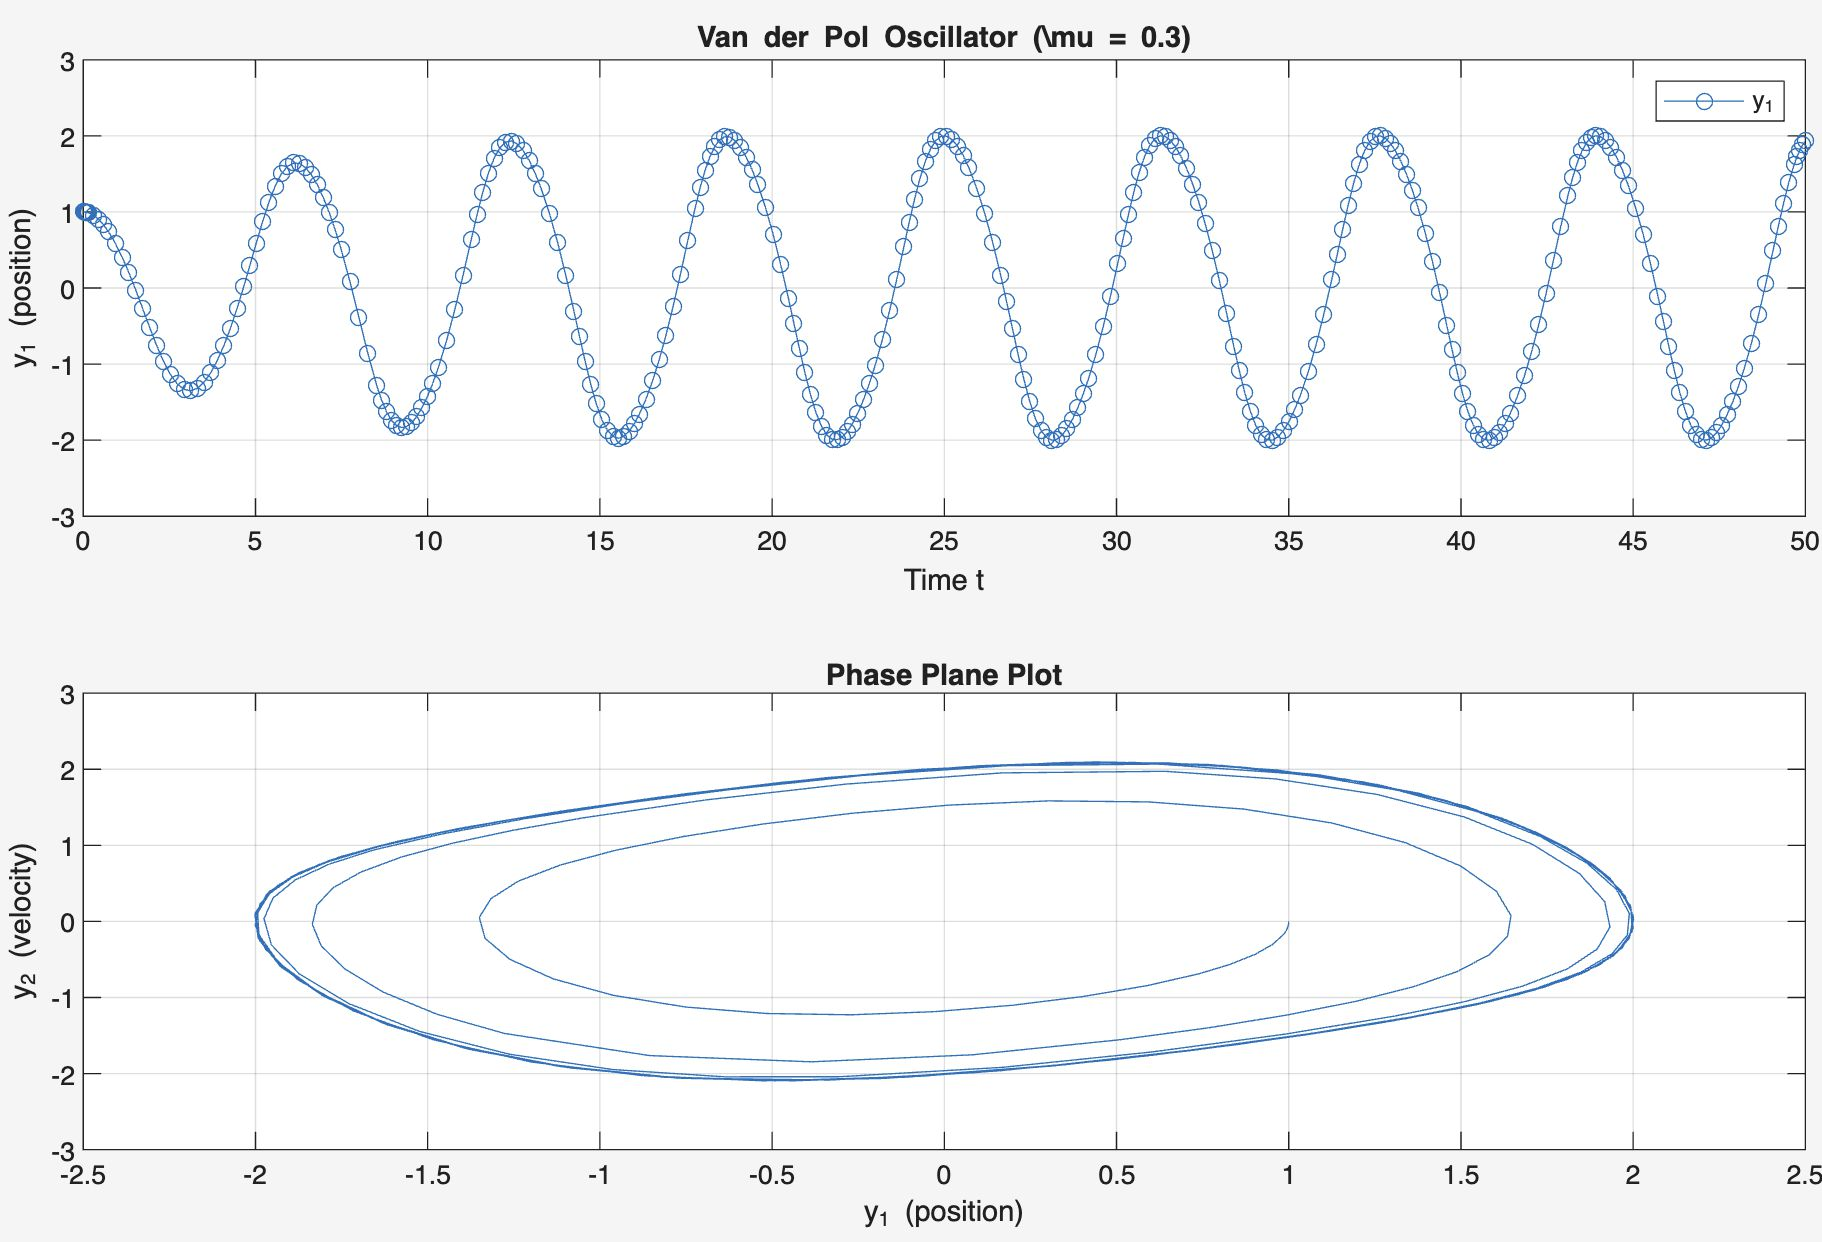
\includegraphics[width=0.45\linewidth]{00_Images/04_chapter/img127.jpg}}
\caption{Van der Pol oscillator: representative waveforms and phase portraits for two parameter settings}
\label{fig:vanderpol_examples}
\end{figure} 

\section{Reed as a Generator}

\subsection{Generator Behavior at Playing Frequency}

The quasi-static description is limited to very low frequencies. Introducing reed dynamics leads to
\[
\frac{d^2 x}{dt^2} + 2\gamma \frac{dx}{dt} + \omega_r^2 (x - x_0)
= \frac{S}{m}(\sigma_1 p_1 + \sigma_2 p_2)
\]
where \( \omega_r \) is the reed resonance frequency. The pressures \( p_1 \) and \( p_2 \) depend nonlinearly on the aperture \( x \), hence the exciter behaves as a nonlinear oscillator. The equilibrium (operating-point) opening follows from the static balance
\[
x = x_0 + (\sigma_1 p_1 + \sigma_2 p_2)\frac{S}{m\omega_r^2}
\]
At playing conditions, flow and pressure vary approximately sinusoidally around this operating point. 

\paragraph{Onset conditions} For oscillations to start, the following conditions must hold:
\[
(-,+): \ \omega < \omega_r
\qquad
X_1 + X_2 > 0
\]
\[
(+,-): \ \omega > \omega_r
\qquad
X_1 + X_2 < 0
\]
\[
(+,+): \ \frac{\omega - \omega_r}{X_1^2 - X_2^2} > 0
\qquad
X_1 - X_2 < 0
\]
where \( X_1 \) and \( X_2 \) are the reactances of the player mouth and the instrument tube, respectively. 

\subsection{Clarinet-type Reed}

For a clarinet-type reed \( (-,+) \), the playing frequency must lie below \( \omega_r \), and the total reactance must be positive. In practice, the largely negative mouth reactance must be compensated by a positive tube reactance, which requires playing sufficiently close to a tube resonance.

\subsection{Brass Instruments}

In a brass instrument played in the \( (+,-) \) configuration, the playing frequency must be above the lip resonances, and the mouth cavity compliance \( X_1 < 0 \) assists the oscillation. In the \( (+,+) \) configuration, the playing frequency will generally be below the lip and horn resonances. 

\subsection{Free Reeds}

Free reeds are a useful model for harmoniums and mouth organs. An idealized free reed consists of a curved metal tongue attached to a thin plate containing an aperture through which the tongue can just pass, and practical realizations exhibit tongue curvature and a plate of appreciable thickness. Their static flow characteristic can be represented by a curve with a preferred operating region. A schematic view of a free reed and a representative static characteristic are shown in figure \ref{fig:free_reed_scheme_characteristic}.

\begin{figure}[!htb]
\centering
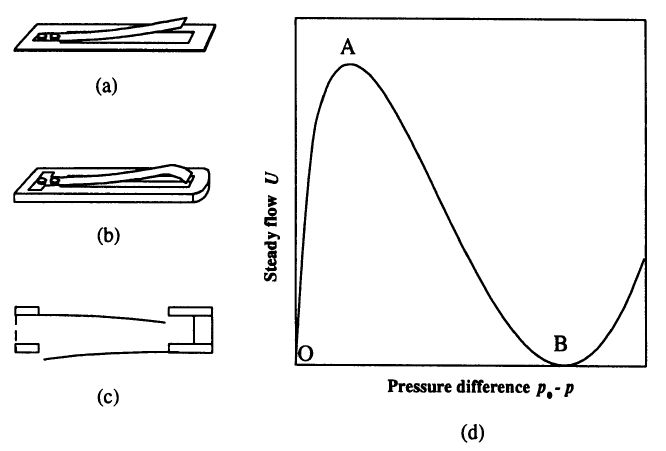
\includegraphics[width=0.8\linewidth]{00_Images/04_chapter/img142.jpg}
\caption{Free reed: geometry and representative static flow characteristic}
\label{fig:free_reed_scheme_characteristic}
\end{figure}

The playing frequency is very close to the reed resonance frequency. The best operating point lies between A and B: for a not too large pressure offset, the admittance is negative and the reed acts as a generator. If the pressure offset becomes large, the working point may move beyond B, decreasing the amplitude of the acoustic volume flow.

\subsection{Mouth Organ}

In a mouth organ, two reeds are coupled by the small air volume between them. The two reeds have opposite behaviors: one operates as \( (-,+) \) and the other as \( (+,-) \), and the resonance frequency of the closing reed is lower than that of the opening reed. When the instrument is blown, the \( (-,+) \) reed sounds, whereas the other reed produces sound when played by suction. 

\begin{figure}[!htb]
\centering
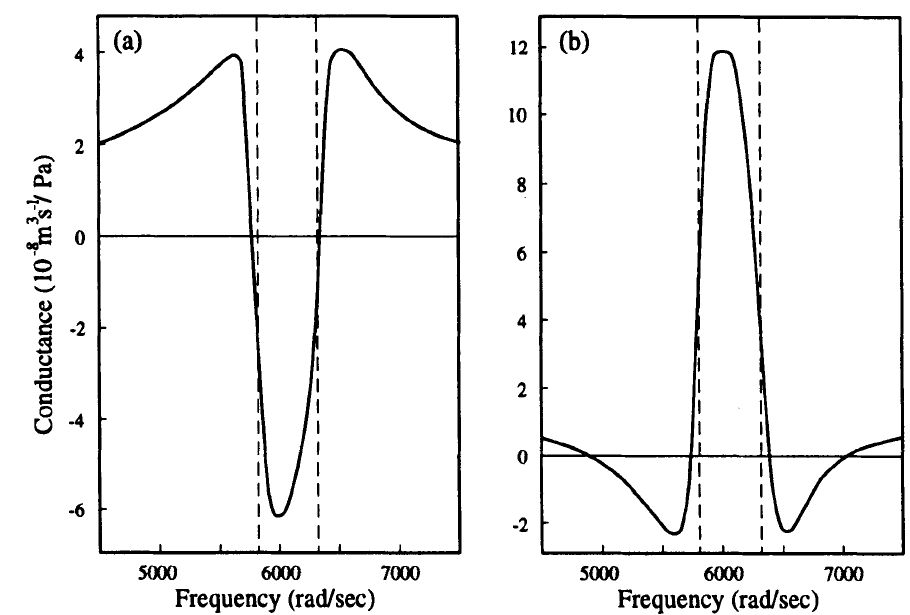
\includegraphics[width=0.8\linewidth]{00_Images/04_chapter/img157.jpg}
\caption{Pitch bending interpreted through the conductance of a coupled-reed model}
\label{fig:pitch_bending_conductance}
\end{figure}

\paragraph{Pitch bending} Pitch bending can be discussed in terms of the acoustic conductance of a coupled-reed model. The conductance behavior underlying pitch bending is illustrated in figure \ref{fig:pitch_bending_conductance}. When the resonance frequency of the closing reed is higher than that of the opening reed, pitch bending becomes possible for the closing reed. Conversely, if the resonance frequency of the closing reed is lower than that of the opening reed, the conductance behavior changes accordingly and pitch bending is not supported in the same way.

\subsection{Generators Coupled to Horns}

For an open cylindrical pipe of length \( L \) and cross-section \( S \), predominantly damped by wall losses, the input impedance can be written as
\[
Z_p = Y_p^{-1}
= \frac{\rho c}{S}
\frac{1 + jH\tan(kL)}{H + j\tan(kL)}
\]
where \( \rho \) is the density, \( c \) is the sound speed, \( k \) is the wavenumber and \( H \) is the height of the impedance maxima relative to \( \rho c/S \). The impedance maxima occur at
\[
\omega_p^{(n)} = \frac{(2n+1)\pi c}{2L}
\]
For an oscillation to grow, the overall system must operate at resonance, meaning that the overall impedance has no imaginary part and the generator overcomes the losses:
\[
\Im(Y_r) = -\Im(Y_p)
\qquad
-\Re(Y_r) > \Re(Y_p)
\]
Since \( \Im(Y_r) > 0 \) for \( (-,+) \) and \( (+,+) \) valves, one needs \( \Im(Y_p) < 0 \), implying an operating frequency slightly below the pipe resonance,
\[
\omega = \omega_p^{(n)} - \delta
\]
Conversely, for a \( (+,-) \) reed, the operating frequency must be slightly above resonance,
\[
\omega = \omega_p^{(n)} + \delta
\]

\section{Large Amplitude Behavior}

The considerations introduced previously are valid when the magnitude of the signal is small enough that a linearized version of the nonlinear reed characteristic can be used. In practice, the pressure excursion in the reed channel can be large, so the linearized characteristic is no longer informative. Even though large-amplitude regimes are generally difficult to treat, useful insights can be gained through an ab initio computation, which follows in time the progressive and regressive pressure waves in the tube and their interaction with the reed.

\subsection{Ab Initio Computation}

A convenient formulation is obtained by introducing dimensionless quantities,
\[
x^{e} = \frac{x}{H}
\qquad
p^{e} = \frac{p}{p_{C}}
\qquad
U^{e} = \frac{U Z_{c}}{p_{C}}
\qquad
Z_{c} = \frac{\rho c}{S_{P}}
\]
together with
\[
y = x^{e} + \gamma
\qquad
\gamma = \frac{p_{0}}{p_{C}}
\]
and the reed parameter
\[
\zeta = \frac{Z_{c} U(p_{A})}{p_{C}}
\]
The parameter \( \zeta \) typically lies between \( 0.3 \) and \( 0.4 \) and influences the attack transient, while the mouth pressure \( p_{0} \) dictates the amplitude and the spectrum. For notational simplicity, the superscripts are omitted in the following.

\paragraph{Progressive and regressive waves} At the pipe entrance, pressure and volume flow can be expressed in terms of progressive and regressive waves,
\[
\begin{aligned}
p &= p^{+} + p^{-} \\
U &= p^{+} - p^{-}
\end{aligned}
\qquad
\begin{aligned}
p^{+} &= \frac{1}{2}(p + U) \\
p^{-} &= \frac{1}{2}(p - U)
\end{aligned}
\]
This corresponds to a \( 45^{\circ} \) rotation of the \((p,U)\) coordinates. Since the reed characteristic provides a nonlinear relation between \( p \) and \( U \), it can be rewritten in the \((p^{+},p^{-})\) coordinates as
\[
p^{+} = G(-p^{-})
\]
where \( G \) is the reed characteristic rotated by \( 45^{\circ} \).

\paragraph{Time-domain formulation} A time-domain analysis of wave propagation in the pipe leads to
\[
p(t) = U(t) + [r \star (p + U)](t)
\]
where \( r(t) \) is the reflection function of the pipe. For a lossless pipe,
\[
r(t) = -\delta(t - \tau)
\]
so that
\[
p(t) = U(t) - p(t - \tau) - U(t - \tau)
\]
Equivalently, the lossless assumption implies
\[
p^{-}(t) = -p^{+}(t - \tau)
\]
and, at the reed,
\[
p^{+}(t) = G(-p^{-}(t)) = G(p^{+}(t - \tau))
\]

\paragraph{Iterative graphical solution} Sampling at \( t = 0, \tau, 2\tau, \ldots \) and denoting the sample index by \( n \), the wave interaction can be obtained iteratively from
\[
p^{-}_{n} = -p^{+}_{n-1}
\qquad
p^{+}_{n} = G(-p^{-}_{n}) = G(p^{+}_{n-1})
\]
A graphical iteration based on these equations yields a sequence converging to a periodic regime, and it captures the emergence of strongly non-sinusoidal waveforms. A graphical construction illustrating the iteration toward the periodic regime is shown in figure \ref{fig:graphical_iteration_solution} and the resulting mouthpiece-pressure waveform can depart strongly from sinusoidal behavior, as illustrated in figure \ref{fig:pressure_vs_square_wave}.

\begin{figure}[!htb]
\centering
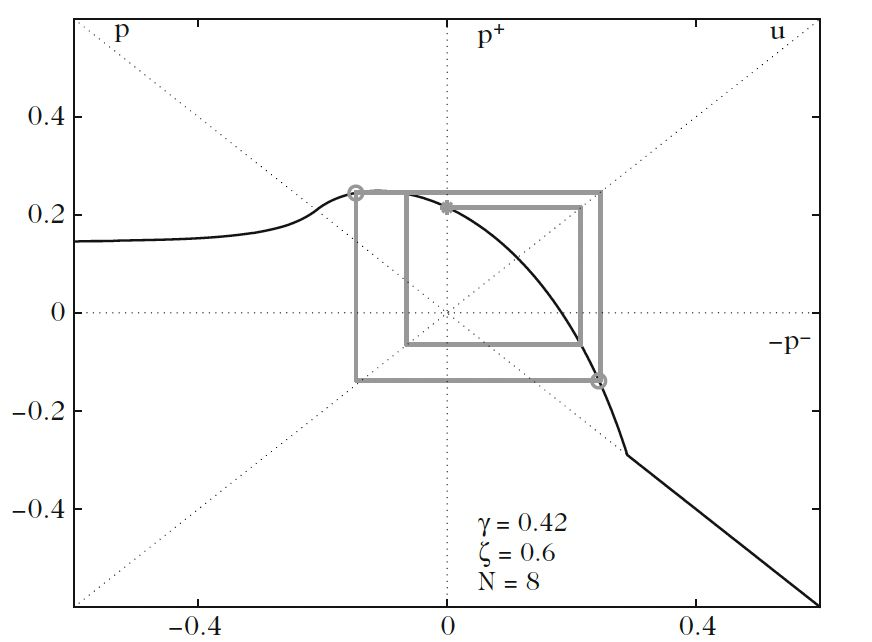
\includegraphics[width=0.6\linewidth]{00_Images/04_chapter/img168.jpg}
\caption{Graphical iteration in rotated coordinates leading to the periodic regime}
\label{fig:graphical_iteration_solution}
\end{figure}

\begin{figure}[!htb]
\centering
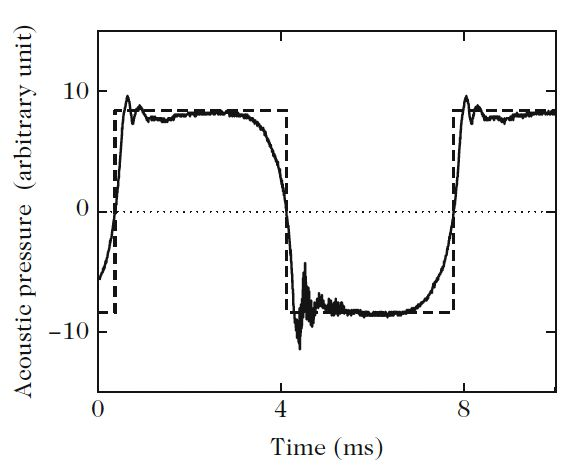
\includegraphics[width=0.6\linewidth]{00_Images/04_chapter/img174.jpg}
\caption{Large-amplitude regime: comparison between computed pressure waveform and an idealized square wave}
\label{fig:pressure_vs_square_wave}
\end{figure}

In the reported examples, increasing \( \zeta \) shortens the transient, while sufficiently small \( \gamma \) leads to convergence toward the static regime. Representative transients of pressure and volume flow for different parameter choices are shown in figure \ref{fig:transients_zeta_gamma}.

\begin{figure}[!htb]
\centering
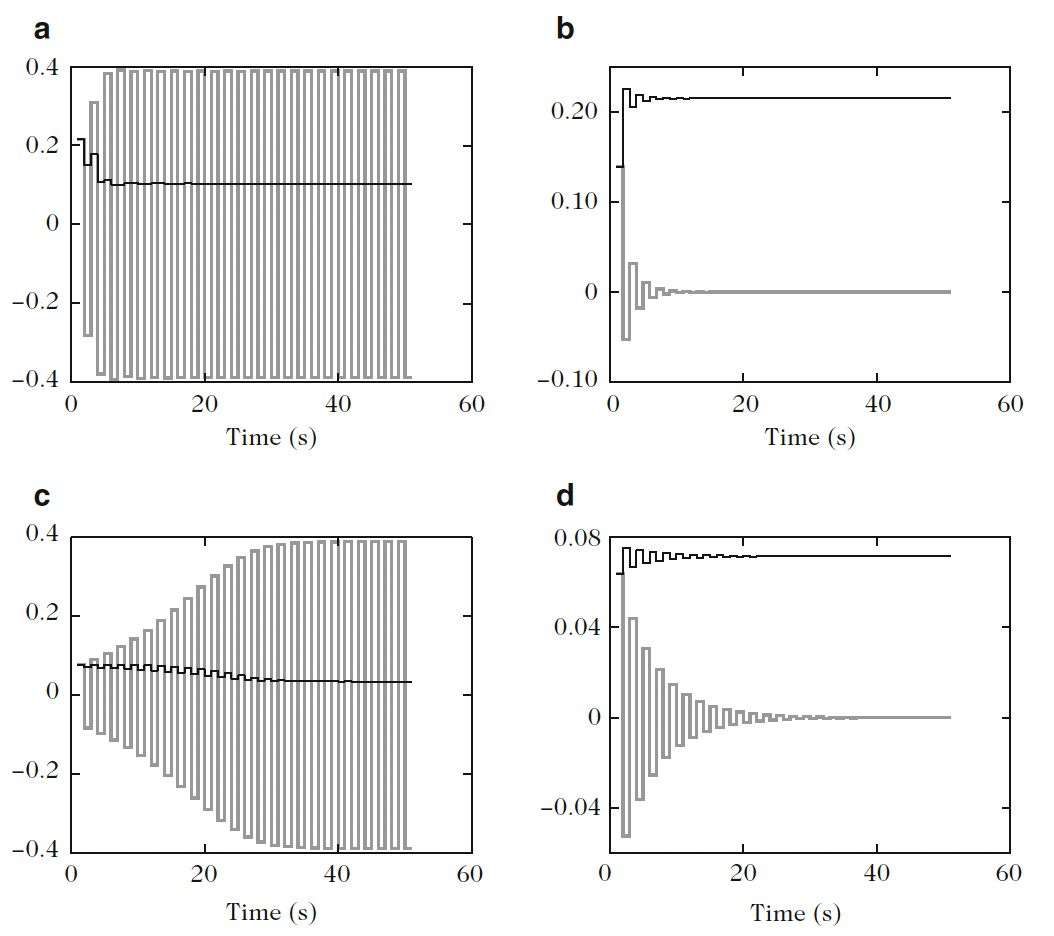
\includegraphics[width=0.7\linewidth]{00_Images/04_chapter/img180.jpg}
\caption{Attack transients of pressure and volume flow for different \(\zeta\) and \(\gamma\)}
\label{fig:transients_zeta_gamma}
\end{figure}

\subsection{Woodwind Single Reeds}

An intuitive view of the large-amplitude regime is obtained by considering the blowing pressure \( p_{0} \). In order for the mouthpiece pressure waveform to be symmetric about \( p_{0} \), the quantity \( p_{0} - p \) must have equal positive and negative excursions, which corresponds to choosing \( p_{0} \) midway between two points on the static characteristic. In this regime, the mouthpiece pressure can switch abruptly between two extreme values, while the volume flow in the two switched states is the same, apart from a finite switching transient. An illustration of switching between two extreme pressure states and the associated transient is shown in figure \ref{fig:single_reed_switching}.

\begin{figure}[!htb]
\centering
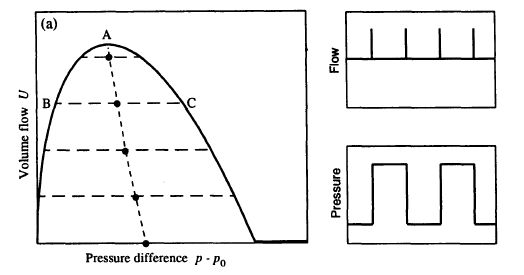
\includegraphics[width=0.7\linewidth]{00_Images/04_chapter/img192.jpg}
\caption{Single-reed large-amplitude regime: switching behavior and switching transient}
\label{fig:single_reed_switching}
\end{figure}

\paragraph{Lossy configuration and load lines} In a lossy configuration, the load lines are not horizontal. The effect of non-horizontal load lines in a lossy configuration is illustrated in figure \ref{fig:lossy_load_lines}.

\begin{figure}[!htb]
\centering
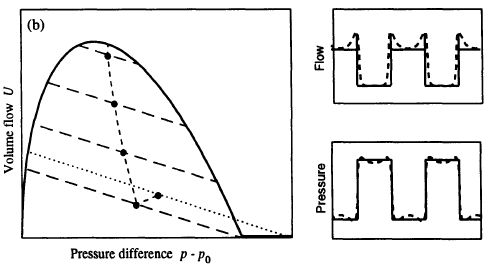
\includegraphics[width=0.7\linewidth]{00_Images/04_chapter/img197.jpg}
\caption{Lossy configuration: load lines and oscillation condition relative to the maximum negative slope}
\label{fig:lossy_load_lines}
\end{figure}

Oscillation can begin only if the load-line slope is smaller than the maximum negative slope of the reed flow characteristic. In that case, the two parts of the flow cycle have different magnitudes, producing a waveform that supplies energy to overcome the losses. Once the reed vibration reaches the beating point, the behavior changes, as indicated by a kink in the blowing-pressure curve.

\subsection{Woodwind Double Reeds}

For woodwind double reeds, the static flow is more complex because of losses in the narrow passage between the two reeds. The resulting characteristic may exhibit hysteresis. A representative hysteretic characteristic and the associated jump in operating point are shown in figure \ref{fig:double_reed_hysteresis_jump}. As the pressure rises from \( O \) to \( A^{\prime\prime} \), the admittance is positive and oscillation cannot begin. When the oscillation reaches \( A^{\prime\prime} \), the flow drops abruptly to \( C \), generating a pulse that propagates along the resonator and returns to the mouthpiece after reflection. The returning pulse lowers \( p_{0} - p \), driving the operating point to \( F \), and the cycle repeats.

\begin{figure}[!htb]
\centering
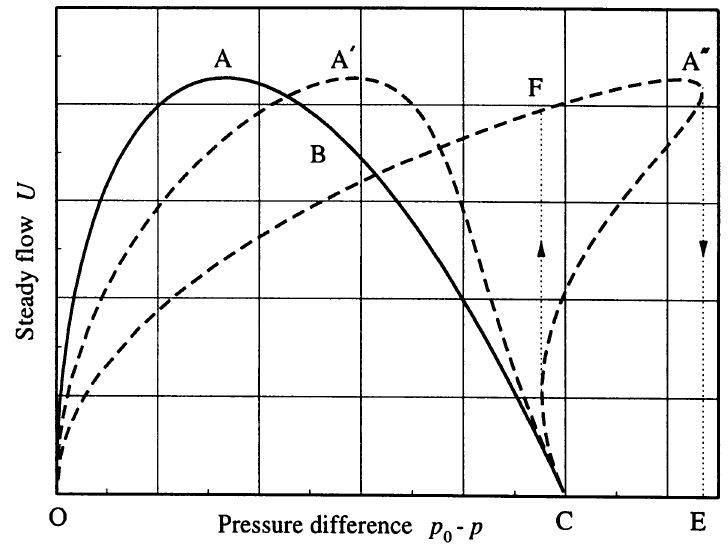
\includegraphics[width=0.7\linewidth]{00_Images/04_chapter/img202.jpg}
\caption{Double reeds: hysteresis in the static characteristic and jump from \(A^{\prime\prime}\) to \(C\)}
\label{fig:double_reed_hysteresis_jump}
\end{figure}

\subsection{Resonant Reeds and Lip Valves}

When a reed is driven at a frequency close to one of its resonances, as in the harmonium, the vibration remains essentially sinusoidal, with the notable exception of an organ pipe, where the reed can strike the shallot. Lip valves also exhibit a fairly sinusoidal behavior. The power produced by the lip generator follows a trend of the form
\[
P \propto p_{0}(p_{0} - p_{T})^{4}
\]
where \( p_{T} \) is the threshold pressure for oscillation onset. The radiated power follows a similar trend, up to losses in the instrument, and in the mid-pressure range, doubling \( p_{0} \) increases the output power by about \( \SI{15}{\decibel} \).

\subsection{Nonlinear Analysis and Harmonic Content}

The relationship between \( p \) and \( U \) is strongly nonlinear. As a consequence, an excitation at angular frequency \( \omega \) generates a flow containing components at \( n\omega \). These components enter the resonator, which behaves linearly, and generate pressure components of the form at the mouthpiece.
\[
p_{n} = Z_{p}(n\omega)U_{n}\sin(n\omega t)
\]
For a given flow, the output pressure is maximized when the system impedance is at a maximum, so instruments excited by pressure-controlled valves tend to operate at frequencies of impedance maxima. In woodwind reeds operating far from reed resonances, multiple pressure components contribute to a rich harmonic spectrum. In a saxophone, with an almost conical bore, the impedance maxima occur at \( n\omega_{1} \), so the returning pressure contains all harmonics. In a clarinet, with an open cylindrical bore, impedance maxima occur at \( (2n-1)\omega_{1} \), so the returning pressure contains only odd harmonics. When reeds operate close to a resonance, the oscillation remains nearly sinusoidal.
